% !TEX root = SegwayDoku.tex
\renewcommand{\autoren}{Valentyn Chepil}
\newpage
\section{Die Hinderniserkennung}
\subsection{Ultraschallsensor}
% \ref{bild_3} zuweisung auf Bild in Text.

\begin{figure}[!h]  % [h] bedeutet, dass das Bild genau an dieser Stelle im Text erscheint
	% mit width=... wird die Größe des Bildes in Prozent der Seitenbreite eingestellt
	\centering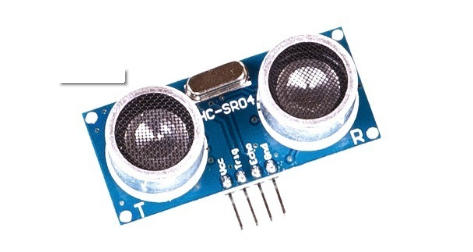
\includegraphics[width=0.5\textwidth]{images/Bild-1-1.png}
	% caption ist die Bildunterschrift, taucht auch im Abbildungsverzeichnis auf
	\caption{Ultraschallsensor \newline(Quelle: funduinoshop.com)}
	\label{bild_1.1} % über das label kann man aus dem Text auf das Bild verweisen
\end{figure}

\textbf{Parameter:}  %fett 
\begin{itemize} 
	\item Modul: HC-SR04 
	\item Preis:  1.50 Doller
\end{itemize}

Die Erkennung vom Hindernis erfolgt über ausgehenden Schallwellen, die sich in kegelförmig Form  ausbreiten. Bei Erreichung des Ziels werden die reflektierende Schallwellen aufgenommen und das Zeig des Reflektion wird ausgemessen. Dadurch erkennt man das Hindernis und den Abstand zu dem. Die Ausbreitung und die reflektierende Schallwellen hängt von verschiedenen Faktoren ab. Sie werden vom Luftdruck, der Umgebungstemperatur, der Luftfeuchtigkeit sowie vom Sende-/Empfangswinkel und der Oberfläche des im Schallkegel befindlichen Objekts
beeinflusst.

\begin{figure}[!h]  % [h] bedeutet, dass das Bild genau an dieser Stelle im Text erscheint
	\centering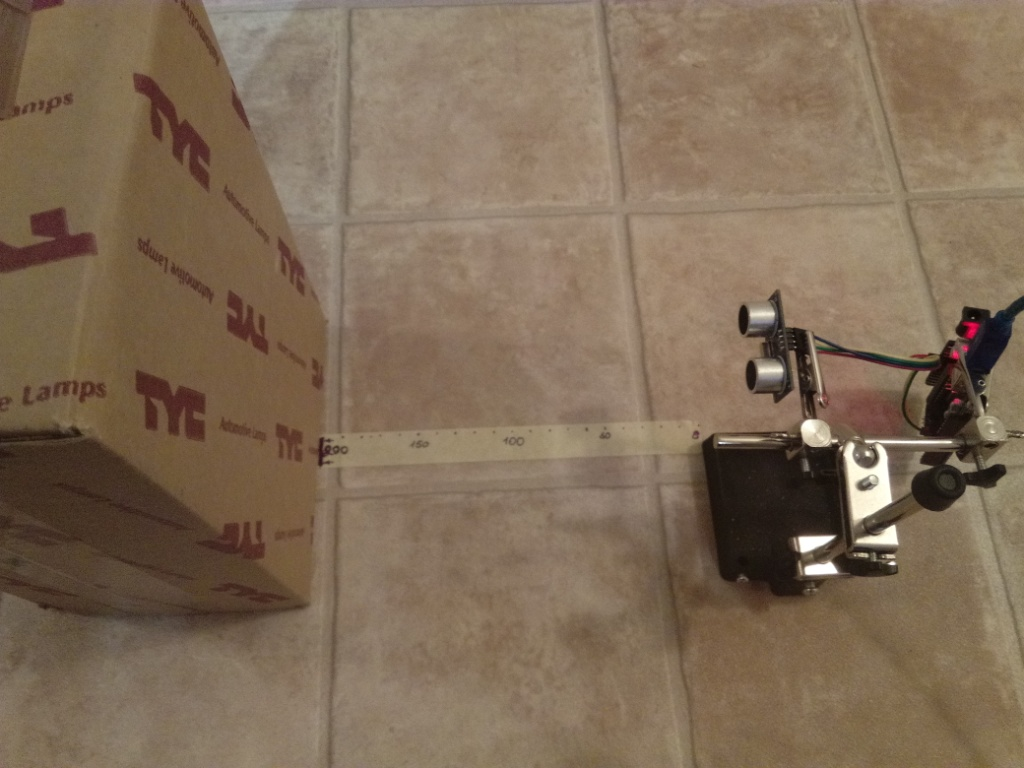
\includegraphics[width=0.6\textwidth]{images/Bild-1.jpg}
	\caption{Entfernungsmessung \newline (Quelle: eigene Darstellung, US-Sensor Messvorgang)}
	\label{bild_1} % über das label kann man aus dem Text auf das Bild verweisen
\end{figure}

\textbf{Vorteile:}  %fett 

Ein größter Vorteil des Ultraschallsensors ist günstiger Preis. Dies ermöglicht die Verwendung von vielen Sensoren bei der Modellbau, was zur präzisen Erfassung der Entfernung zu Hindernissen und Objekten in der Umgebung führt. Kann man in der Abbildung \ref{bild_1} sehen.

\par\bigskip %leere zeile
\textbf{Nachteile:}  %fett 

Ein Hindernis oder Objekt kann nicht genau geortet werden, sondern man kann nur feststellen, dass es sich in der gemessenen Entfernung innerhalb des Schallkegels befindet. Kann man in der Abbildung \ref{bild_2} sehen.

\begin{figure}[ht]  % [h] bedeutet, dass das Bild genau an dieser Stelle im Text erscheint
	\centering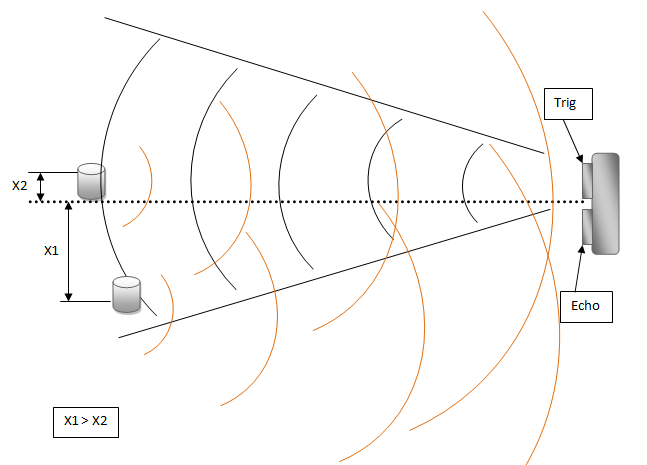
\includegraphics[width=0.6\textwidth]{images/Bild-2.png}
	\caption{Positionierung in Messbereich \newline (Quelle: eigene Darstellung)}
	\label{bild_2} % über das label kann man aus dem Text auf das Bild verweisen
\end{figure}

Bei mehrere Objekten vor Schallwelle wird der Abstand zum nächstliegenden Hindernis gemessen und die weit liegender Objekte werde einfach nicht erkannt. Kann man in der Abbildung \ref{bild_3} sehen.


\begin{figure}[ht]  % [h] bedeutet, dass das Bild genau an dieser Stelle im Text erscheint
	\centering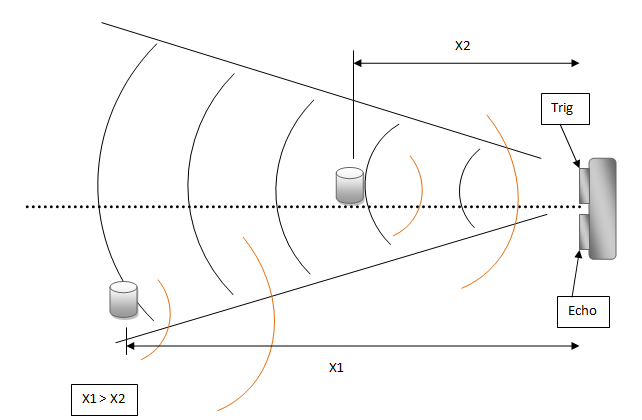
\includegraphics[width=0.6\textwidth]{images/Bild-3.png}
	\caption{Positionierung in Messbereich \newline (Quelle: eigene Darstellung)}
	\label{bild_3} % über das label kann man aus dem Text auf das Bild verweisen
\end{figure}

Als Nachteil kann man nennen die geringe Reichweite (ca. 3m) des Ultraschalls und  der geringen Ausbreitungsgeschwindigkeit des Schalls.

Große Probleme bekommt man auch aus den Reflektionseigenschaften der Schallwellen. Besonders bei weichen Materialien und spitzen-förmigen Oberflächen,
Oberflächenerkennung erfasst das Sensor auch schleicht. Das kann man in der Abbildung \ref{bild_4} sehen.

\begin{figure}[!h]  % [h] bedeutet, dass das Bild genau an dieser Stelle im Text erscheint
	\centering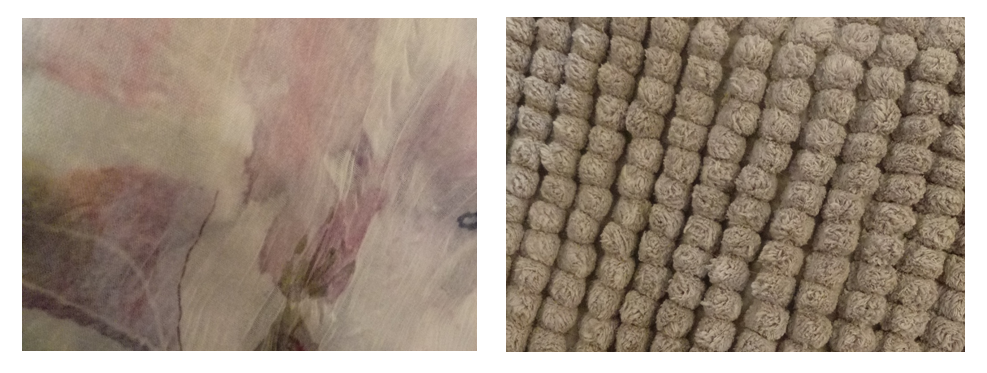
\includegraphics[width=0.8\textwidth]{images/Bild-4-5.png}
	\caption{Weiche und spitzen-förmige-weiche Oberflächen \newline(Quelle: eigene Darstellung,Frauen-Halsschal und Teppich)}
	\label{bild_4}
\end{figure}

\begin{figure}[!h]  % [h] bedeutet, dass das Bild genau an dieser Stelle im Text erscheint
	\centering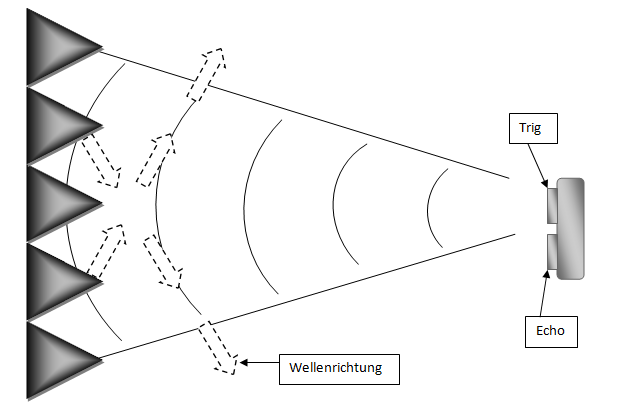
\includegraphics[width=0.55\textwidth]{images/Bild-6.png}
	\caption{Spitzen-förmige Oberflächen\newline(Quelle: eigene Darstellung, z.B: Kanten)}
	\label{bild_6}
\end{figure}

\begin{figure}[!h]  % [h] bedeutet, dass das Bild genau an dieser Stelle im Text erscheint
	\centering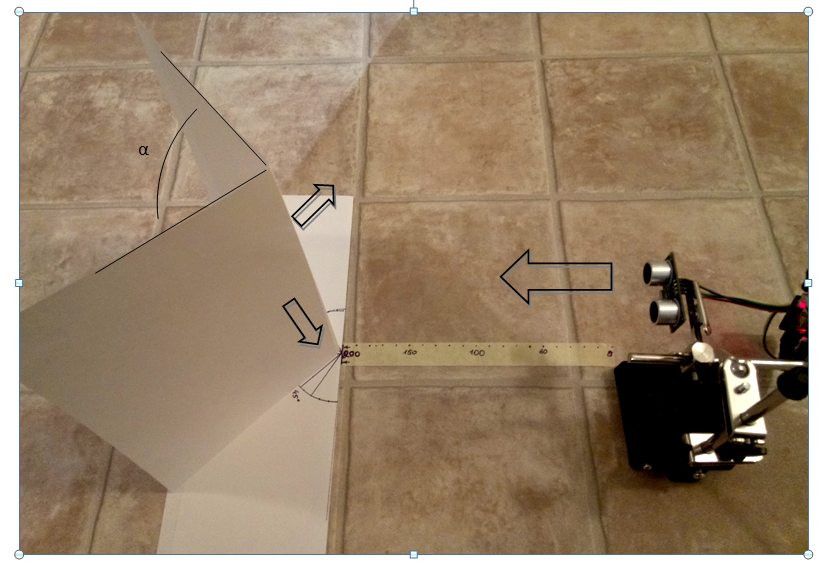
\includegraphics[width=0.5\textwidth]{images/Bild-7.png}
	\caption{Öffnungswinkel (Quelle: eigene Darstellung)}
	\label{bild_7} % über das label kann man aus dem Text auf das Bild verweisen
\end{figure}

Wird das Winkel des Schallkegels größer seinem Öffnungswinkel auf eine ebene Wand, so erreicht die Reflektion den aussendenden Sensor nicht. Kann man am Abbildung \ref{bild_7} sehen.

\subsection{Laser Sensor - Variante 1}

\begin{figure}[!h]  % [h] bedeutet, dass das Bild genau an dieser Stelle im Text erscheint
	\centering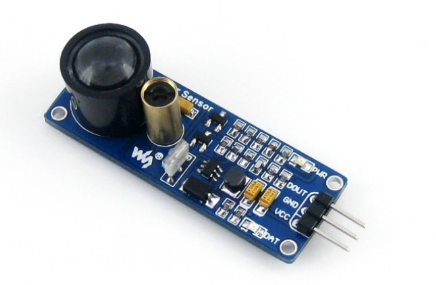
\includegraphics[width=0.6\textwidth]{images/laser-sensor.png}
	\caption{Laser-Sensor (Quelle: waveshare.com)}
	\label{laser-sensor} % über das label kann man aus dem Text auf das Bild verweisen
\end{figure}

\textbf{Parameter:}  %fett 
\begin{itemize}
\item Modul: 
\item Chip-Name: PT1301
\item Preis: 10.79 Doller
\item Quelle: https://www.waveshare.com/Laser-Sensor.htm
\end{itemize}
\begin{figure}[!h]  % [h] bedeutet, dass das Bild genau an dieser Stelle im Text erscheint
	\centering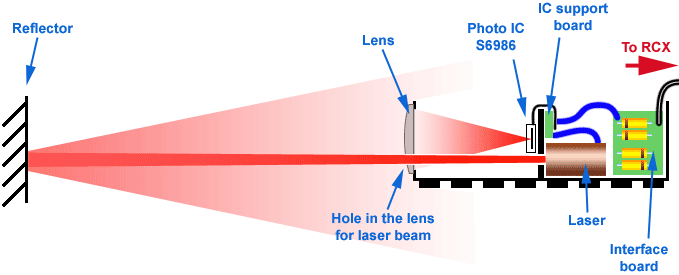
\includegraphics[width=0.9\textwidth]{images/laser-sensor1.png}
	\caption{ \ Aufbau der Sensors (Quelle:philohome.com)}
	\label{laser-sensor1} % über das label kann man aus dem Text auf das Bild verweisen
\end{figure}

\par\bigskip %leere zeile
\textbf{Vorteile:}  %fett 

\par\bigskip %leere zeile
\textbf{Nachteile:}  %fett 




\pagebreak

\subsection{Laser Sensor - Variante 2}
\begin{figure}[htbp!]  % [h] bedeutet, dass das Bild genau an dieser Stelle im Text erscheint
	\centering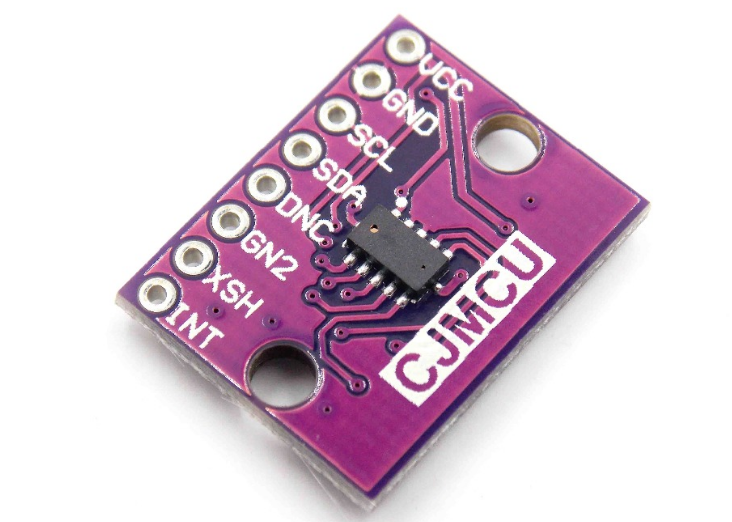
\includegraphics[width=0.6\textwidth]{images/laser-sensor_v2.png}
	\caption{ \ Laser-Sensor-VL53L0X (Quelle: ebay.de)}
	\label{laser-sensor_v2} % über das label kann man aus dem Text auf das Bild verweisen
\end{figure}

\textbf{Parameter:}  %fett 

\begin{itemize}
\item Modul: CJMCU-530
\item Chip-Name: VL53L0X
\item Preis: 4,84 Doller
\end{itemize}

\par\bigskip %leere zeile
\textbf{Vorteile:}  %fett 

\par\bigskip %leere zeile
\textbf{Nachteile:}  %fett 

\subsection{Infrarot Sensor}

\begin{figure}[ht]  % [h] bedeutet, dass das Bild genau an dieser Stelle im Text erscheint
	\centering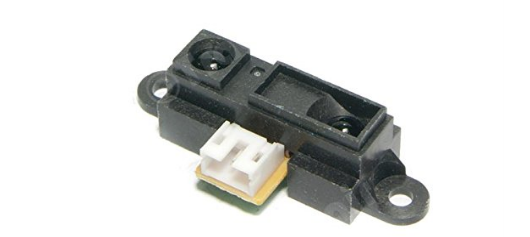
\includegraphics[width=0.8\textwidth]{images/infrarot.png}
	\caption{ \ Infrarot-Sensor  (Quelle: amazon.de)}
	\label{infrarot} % über das label kann man aus dem Text auf das Bild verweisen
\end{figure}

\textbf{Parameter:}  %fett 

\begin{itemize}
\item Modul: GP2Y0A21YK0F
\item Preis: 3,11 Doller
\item Kommunikation: Analog Output Voltage (typischerweise 0,4 bis 2,3 V Range)
\item Betriebstemperatur:-10 bis + 60 °C
\item Minimale Messdistanz = 10 cm
\item Maximale Messdistanz = 80 cm
\item Reaktionszeit = 38 ± 10 ms
\end{itemize}

\par\bigskip %leere zeile
\textbf{Vorteile:}  %fett 

\par\bigskip %leere zeile
\textbf{Nachteile:}  %fett 

Durch die Anwendung der Triangulatio haben das Reflexionsverhalten des Gegenstands, die Umgebungstemperatur und die Betriebsdauer einen sehr geringen Einfluss auf die Abweichung der Messung. Die analoge Ausgangsspannung des Abstandssensors hängt von der gemessenen Entfernung ab. Somit kann der Sensor auch als Näherungssensor genutzt werden.

Produktinformationen:

Abstandsmessbereich 10cm – 80cm
Betriebsspannung 5V DC
Stromaufnahme 40 mA
Sensorausgang: alnaloge Spannung
Ausgangsspannung: ca. 0.4V bei 80cm, ca. 2.3V bei 10cm
Ansprechzeit: 39ms
Betriebstemperatur: -10°C bis +60°C
Abmessung: 29,5*13*13,5mm
Lieferumfang:

1 SHARP IR-GP2Y0A21YK0F Distanz Sensor
1 Anschlusskabel mit Stecker
Einfache Verwendung durch Mikrocontroller, so wie Arduino , 8051, AVR, PIC, DSP, ARM, MSP430, PLC,TTL-Logik

%Weitere Details zum Sensor im Datenblatt: %http://www.sharpsma.com/webfm_send/1489

Dieses Sensor sendet ein Strahl des Infrarot-Licht auf ein Objekt und wartet  reflektierte Licht zurück kommt.